\chapter{Umsetzung}

Umgesetzt wurde die Aufgabe im wesentlichen aus drei Teilen: 
\begin{itemize}
	\item Einer SQL-Datenbank mit realit\"atsnahen Tabellen 
	\item Einer Ontologie 
	\item Einem ausf\"uhrbaren Programm mit Grafischer Benutzungsoberfl\"ache

\end{itemize}

\section{Datenbank}

Bei der Datenbank wurde auf eine gew\"ohnliche relationale Datenbank zur\"uckgegriffen, da im wesentlichen nur die g\"angigsten SQL-Befehle benutzt werden. Da es bereits gute Erfahrungen im Team mit MySQL gab, wurde diese Datenbank verwendet. 

Die Datenbank enth\"alt im wesentlichen Informationen die ein Hochschulsportberater ebenfalls nachschlagen w\"urde. Die wichtigsten Informationen sind:
\begin{itemize}
\item Angebotene Sportarten
\item Trainingszeiten
\item Veranstaltungsort
\item H\"ohe der Teilnehmergeb\"uhr
\end{itemize} 
Das genaue Datenbankmodell kann der Abbildung \ref{fig:Datenbank-Design} entnommen werden.

\begin{capfigure}[Datenbank-Design]
	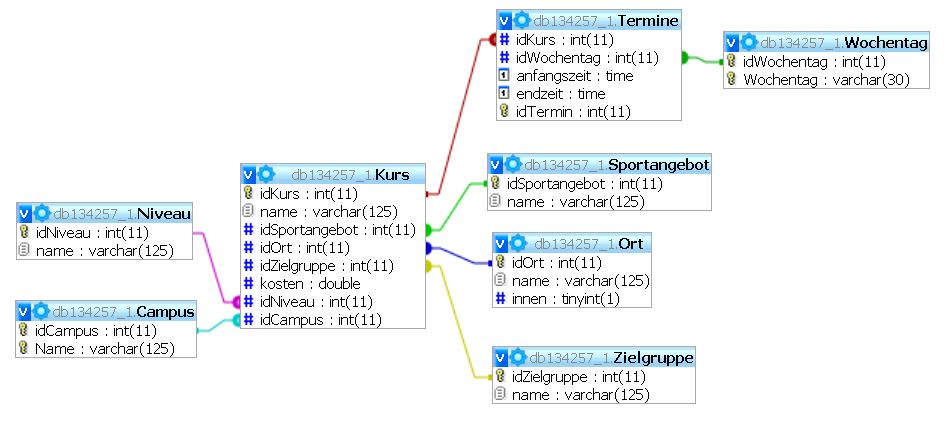
\includegraphics[width=\textwidth]{images/db_design}
\end{capfigure}

\newpage

\section{Ontologie}
%\TODO{[PRIO:SOFORT] Komplett neu machen}
Die Erstellung der Ontologie wird mit \gls{protege} durchgef\"uhrt. \gls{protege} erm\"oglicht nur die Verwendung von OWL-DL. OWL-Full wird nicht unterst\"utzt, daher m\"ussen gewisse Einschr\"ankungen ber\"ucksichtigt werden. Beispielsweise kann man keine Komplementklassen erstellen. 

Des Weiteren sollte man immer bedenken, dass eine Ontologie ein Open-World-Szenario darstellt. Im Speziellen kann man nur nach dem Vorhandensein eines Kriteriums abfragen.

Im Laufe dieses Abschnitts wird erl\"autert, wie die Ontologie erstellt wurde. Im Besonderen werden unsere Entscheidungen bei der Umsetzung begr\"undet und deren Folgen erkl\"art.

\subsection{Grobe Unterteilung der Ontologie}
Zuerst wird die Klasse \textit{Sport} erstellt. Diese Klasse enth\"alt die beiden Unterklassen \textit{Einzelsport} und \textit{Teamsport}. Da wir uns bei den Sportarten daf\"ur entschieden haben, dass eine Sportart entweder Einzelsport oder Teamsport ist macht diese Unterteilung am meisten Sinn. Nat\"urlich erm\"oglicht diese L\"osung nicht, dass eine Sportart zugleich Einzelsport als auch Teamsport ist. Dies ist aber kein Problem, da es in unserem Szenario nicht vorkommt.

Bei der Darstellung der Ontologie lassen wir die Ebene \textit{Thing} aus Gr\"unden der \"Ubersichtlichkeit weg.
Die Ontologie sieht jetzt wie folgt aus:
\begin{capitemize}[Ontologie - Grobe Unterteilung der Ontologie - 1]
		\item Sport
			\begin{itemize}
				\item Einzelsport
				\item Teamsport
			\end{itemize}
\end{capitemize}

Als N\"achstes legen wir die Klassen \textit{Ziele} und \textit{Koerperliche\_Einschraenkungen} an. Diese beiden Klassen dienen dazu, die Eigenschaften \textit{Ziele} und \textit{Koerperliche\_Einschraenkungen} abzubilden. Beide Klassen werden noch mit den jeweiligen Unterklassen, die die m\"oglichen Optionen darstellen erg\"anzt.

Danach sieht die Ontologie wie folgt aus:
\begin{capitemize}[Ontologie - Grobe Unterteilung der Ontologie - 2]
	\item Koerperliche\_Einschraenkungen
		\begin{itemize}
				\item Armbereich
				\item Beinbereich
				\item Hoehenangst
		\end{itemize}
	\item Sport
		\begin{itemize}
			\item Einzelsport
			\item Teamsport
		\end{itemize}
	\item Ziele
		\begin{itemize}
				\item Fitness
				\item Freizeitvergnuegen
				\item SelfDefense
				\item Sozialkontakte
				\item Wettbewerb
		\end{itemize}
\end{capitemize}

Damit sind die Klassen soweit fertig. Die Klassen Koerperliche\_Einschraenkungen und Ziele wurden in dieser Art angelegt, da sie optional sind. Ein Sport muss keine Verkn\"upfung zu diesen Klassen haben. 

%Damit sind die Klassen soweit fertig. Beide Klassen wurden in dieser Art angelegt, da sie optional sind. Ein Sport muss keine Verkn\"upfung zu diesen Klassen haben. \TODO{Ich versteh was du meinst, aber erst beim 2ten Lesen. Bitte umformulieren.} Jetzt werden noch die Object Properties dazu wie folgt angelegt:

Jetzt werden noch die Object Properties dazu wie folgt angelegt: 

\begin{capitemize}[Properties - hatZiel und ungeeignetBei]
	\item hatZiel
		\begin{itemize}
			\item Domains: \textit{Sport}
			\item Ranges: \textit{Ziele}
		\end{itemize}
	\item ungeeignetBei
		\begin{itemize}
			\item Domains: \textit{Sport}
			\item Ranges: \textit{Koerperliche\_Einschraenkungen}
		\end{itemize}
\end{capitemize}

Nun lassen sich die Ziele und Einschr\"ankungen mit den Sportarten verbinden. Ein Problem ergibt sich mit dieser Variante allerdings noch, man kann nicht nach Sportarten suchen die explizit keine Einschr\"ankungen haben. Bei den Zielen gibt es dieses Problem ebenfalls, allerdings spielt es hier keine Rolle, da eine Suche nach Sportarten, die explizit keine Ziele haben keinen Sinn ergibt. Bei den Einschr\"ankungen muss allerdings eine L\"osung her. Da in einem Open-World-Szenario nur nach dem Vorhandensein gefragt werden kann, haben wir uns dazu entschieden noch die Unterklasse \textit{Keine} bei den K\"orperlichen Einschr\"ankungen zu erg\"anzen. Jetzt hat man die M\"oglichkeit, auch Sportarten zu suchen, die bei keiner Einschr\"ankung ungeeignet sind.

Bei den Sportarten muss jetzt jede Sportart die Object Property \textit{ungeeignetBei} verwenden. Dies gilt auch, wenn die Sportart bei beliebigen K\"orperlichen Einschr\"ankungen geeigntet ist. Hierfür wird die oben genannte Unterklasse \textit{Keine} eingesetzt. F"ur die Object Property \textit{hatZiel} m"ussen nur die Ziele umgesetzt werden, nach denen explizit gesucht wird.


Als n"achstes wurden die Eigenschaften umgesetzt, die abfragen ob es sich um Wassersport, Kampfsport, Wassersport oder Sportarten mit K"orperkontakt handelt:

\begin{capitemize}[Properties - istExotisch, istKampfsport, istKoerperkontakt, istWassersport]
	\item istExotisch
		\begin{itemize}
			\item Domains: \textit{Sport}
			\item Ranges: \textit{Boolean}
		\end{itemize}
	\item istKampfsport
		\begin{itemize}
			\item Domains: \textit{Sport}
			\item Ranges: \textit{Boolean}
		\end{itemize}
	\item istKoerperkontakt
		\begin{itemize}
			\item Domains: \textit{Sport}
			\item Ranges: \textit{Boolean}
		\end{itemize}
	\item istWassersport
		\begin{itemize}
			\item Domains: \textit{Sport}
			\item Ranges: \textit{Boolean}
		\end{itemize}
\end{capitemize}

Dies sind Eigenschaften von Sportarten, die mit einem Boolean-Wert abgefragt werden. Wir haben die Klasse Boolean selbst mit den Unterklassen \textit{True} und \textit{False} definiert. Der Grund hierf\"ur ist dass Klassen keine Data-Properties haben. Bei Object-Properties ist es nur m\"oglich Relationen zwischen Klassen darzustellen.  

\subsection{\"Aquivalenzklassen}

Um die Ontologieprobleme in den Szenarien zu l\"osen, wurden in der Ontologie bereits \"Aquivalenzklassen beschrieben. 
Hierzu geh"oren die Ziele (z. B. FitnessZiel, FreizeitvergnuegenZiel) und die Eignung bei K"oerperlichen Einschr"ankungen.
Die Äquivalenzklassen vereinfachen die Query. Zum Beispiel wurde \textit{Sport and (not (ungeeignetBei some Beinbereich))} als "Aquivalenzklasse \textit{GeeignetBeiBeinbereichKE} umgesetzt. In der Umsetzung des Programms wurden die Queries allerdings in voller L"ange erstellt, so dass die Abfrage keine "Aquivalenzklassen mehr benutzt. 

%\TODO{Ich habe die Ontologie ja nachtr\"aglich noch erweitert. Es ist jetzt die Frage, wie wir diese \"Anderungen rein nehmen. Meiner Meinung ist es das Beste, wenn du die Personen und neuen Properties kurz erw\"ahnst und dann auf das entsprechende Kapitel oder Abschnitt verweist. das m\"usste mit \textbackslash nameref gut gehen. }

Um verschiedene Personenarten f"ur die GUI dauerhaft speichern zu k"onnen, haben wir uns "uberlegt, die Ontologie mit Personengruppen (Klasse \textit{Person}) wie \textit{zahlende\_Person} und \textit{eingeschraenkte\_Person} zu erweitern. Als dazugeh"orende Properties wurden will\_zahlen (Boolean) und hat\_Einschraenkung (Koerperliche\_Einschraenkungen) noch als Properties eingeführt. Weitere Details zur Benutzung der Personenarten befinden sich im Kapitel "`\nameref{cha:sprunge}"'.

\section{Programm}

Dieser Abschnitt geht zuerst auf die Entscheidung zum Aufbau der graphischen Oberfl\"ache ein und behandelt danach die technischen Aspekte des Programms. 

\subsection{Entscheidung zum Aufbau der graphischen Oberfl\"ache}
Bei der Gestaltung der GUI, wurde sich daf\"ur entschieden, dass der Benutzer zu jedem Zeitpunkt m\"oglichst alle Auswahlm\"oglichkeiten vor Augen hat und dass er, ebenfalls zu jedem Zeitpunkt, eine Liste mit den Sportarten erhalten kann, die zu seinen Auswahlkriterien passen.

Die Gr\"unde f\"ur diese Entscheidungen sind zum einen die Benutzerfreundlichkeit. Durch diesen Aufbau soll der Benutzer aufgefordert werden, m\"oglichst viele Auswahlkriterien auszuprobieren, da er sofort testen kann, welche Auswirkungen diese auf die Auswahl der Sportarten hat. Dies hat den Vorteil, dass der Benutzer die Kriterien mit, einer f\"ur ihn, hohen Priorit\"at setzen kann und unanger\"uhrt l\"asst, w\"ahrendem er die Kriterien mit einer, f\"ur ihn, niedrigen Priorit\"at schnell und einfach \"andern kann. Ein konkretes Beispiel hierf\"ur w\"are z.B. die Sportart Klettern. F\"ur einige Benutzer ist die H\"ohenangst nur ein leichtes Problem, f\"ur einige andere ist sie un\"uberwindlich. Somit haben die Benutzer mit leichter H\"ohenangst, die M\"oglichkeit die angebotenen Sportarten mit oder ohne H\"ohenangst zu vergleichen, w\"ahrend jene mit starker H\"ohenangst das Kriterium ausw\"ahlen und nicht mehr deaktivieren.

Ein anderer Grund f\"ur diese Entscheidung war die Tatsache, dass unsere Szenarien wenige Spr\"unge von einem Schritt zu einem anderen beinhalten. Deshalb haben wir uns dagegen entschieden eine Frage nach der anderen abzuhandeln, wie die Szenarien dies eigentlich vorsehen und was bei mehreren Spr\"ungen wohl auch einfacher umzusetzen gewesen w\"are. Nichtsdestotrotz wird im Kapitel \ref{cha:sprunge}. \nameref{cha:sprunge} erl\"autert wie die Spr\"unge aus unseren Szenarien dargestellt werden, aber auch wie mehrere dieser Spr\"unge umgesetzt werden k\"onnten, obwohl der Benutzer nach wie vor s\"amtliche Optionen vor Augen hat und m\"oglichst wenig an Flexibilit\"at einb\"ußt.

\subsection{Aufbau der graphischen Oberfl\"ache}

Bei der Abbildung \ref{fig:Hauptfenster} handelt es sich um das Hauptfenster, in dem der Benutzer die M\"oglichkeit hat seine Auswahlkriterien festzulegen, die Suche zu starten sowie die vorgeschlagen Sportarten einzusehen und Informationen \"uber diese zu erhalten. Bei den Auswahlkriterien handelt es sich um jene, die ben\"otigt werden, um die Fragen aus den Szenarien zu beantworten.

Bei der Abbildung \ref{fig:Auswahl der Zeiten} handelt es sich um einen "`Stundenplan"', in dem der Benutzer die Zeitr\"aume festlegen kann, in denen er w\"ochentlich Sport treiben will. 

%\begin{capfigure}[Hauptfenster]%
%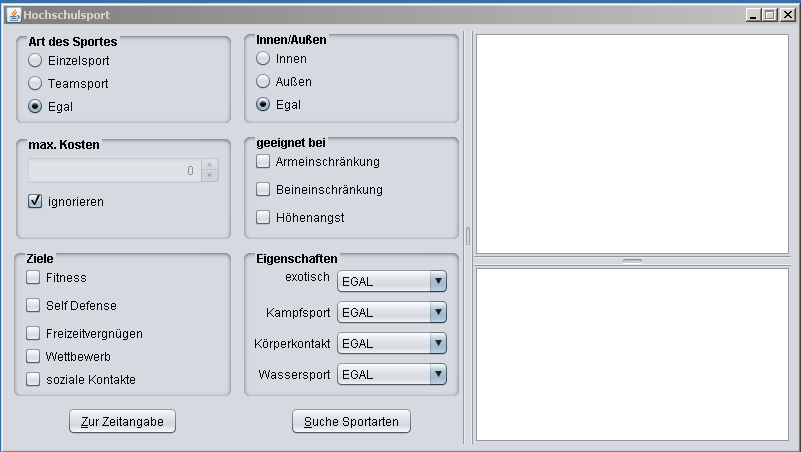
\includegraphics[width=\textwidth]{images/gui.png}%
%\end{capfigure}

%\begin{capfigure}[Auswahl der Zeiten]%
%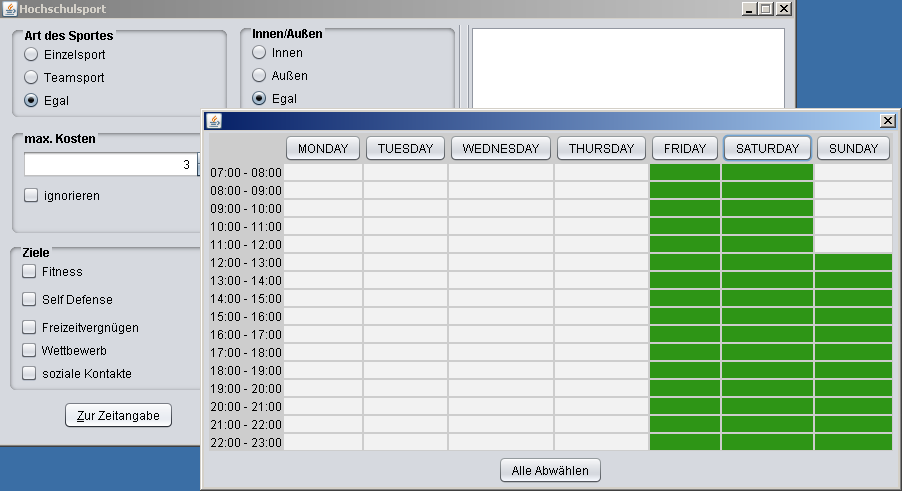
\includegraphics[width=\textwidth]{images/guizeit.png}%
%\end{capfigure}

\begin{figure}[p]
\centering
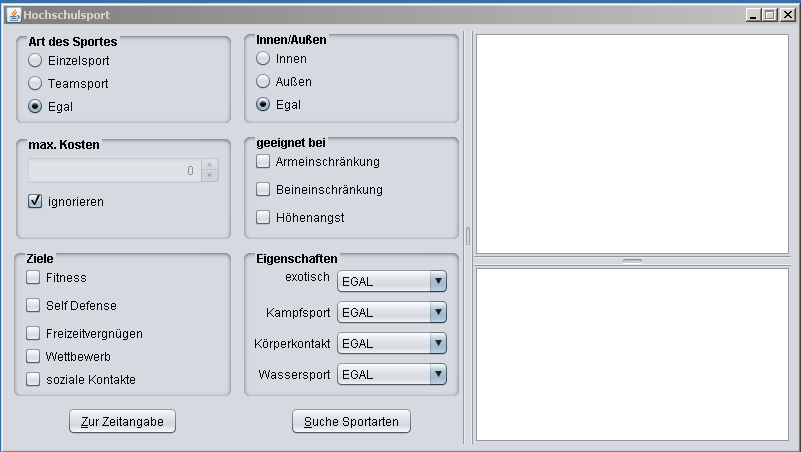
\includegraphics[width=\textwidth]{images/gui.png}%
\caption{Hauptfenster}
\label{fig:Hauptfenster}
\end{figure}

\begin{figure}[p]
\centering
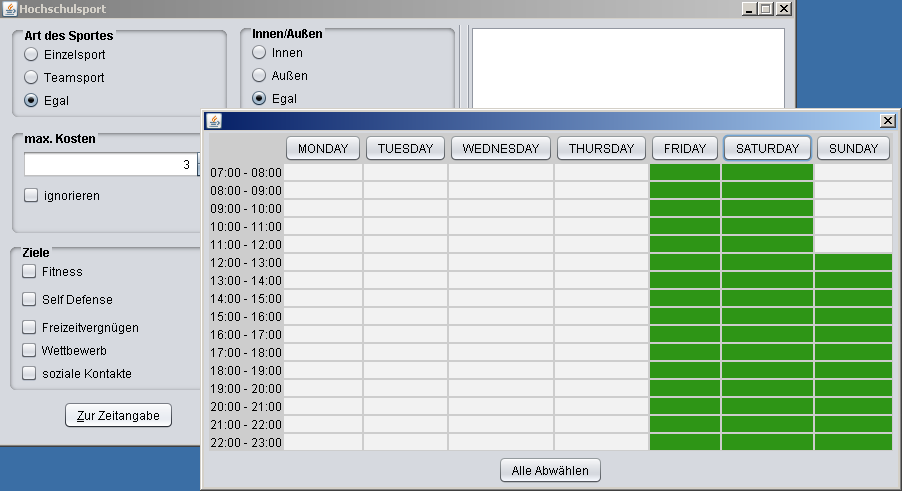
\includegraphics[width=\textwidth]{images/guizeit.png}%
\caption{Auswahl der Zeiten}
\label{fig:Auswahl der Zeiten}
\end{figure}
\newpage
\subsection{Technische Umsetzung}
Das Programm wurde mit Java geschrieben und benutzt die Semantic Web OWL API \autocite{semweb:owlapi} als Verbindung zur Ontologie. Beim benutzten Reasoner handelt es sich um HermIT\autocite{krr:hermit}. Die Verbindung zur Datenbank wird durch einen JDBC-Treiber\autocite{oracle:jdbc} realisiert.

Beim Ausf\"uhren der Suche wird zun\"achst eine Menge mit s\"amtlichen verf\"ugbaren Sportarten erstellt, die daraufhin nach Bedarf gefiltert wird. Der Einfachheit halber wird f\"ur jedes Auswahlkriterium, falls dieses nicht ignoriert werden soll, eine Query ausgef\"uhrt, die die Menge mit den Sportarten weiter filtert. Jede Query hat folgenden, gleichen Aufbau\footnote{UML angelehnte Schreibweise \lstinline[language=Java]"  operation(arg list) : return type" \autocite{kow:umlclass}} \lstinline[language=Java]"query(Sportarten) : gefilterte_Sportarten". Dies bedeutet, dass eine Query eine Menge von Sportarten enth\"alt und nach einem bestimmten Auswahlkriterium filtert, um dann die gefilterte Menge zur\"uckzugeben. Durch den jeweils gleichen Aufbau ergibt sich der Vorteil, dass die Reihenfolge der Queries keine Rolle spielt, und sie demnach auch bei Bedarf \"ubersprungen werden k\"onnen. Das \"Uberspringen von Queries wird ben\"otigt, da jedes Auswahlkriterium vom Benutzer ignoriert werden kann und somit keinen Einfluss auf den Auswahlprozess nimmt.

Das Listing \ref{lst:filtern} zeigt das Filtern an einem konkreten Beispiel. In einem ersten Schritt werden die Sportarten abgefragt. Danach werden die einzelnen Queries durchlaufen, wobei immer abgefragt wird, ob das entsprechende Auswahlkriterium nicht ignoriert werden soll. Im Beispiel wird der nach dem maximalen Preis und den Zielen gefiltert. Es sei noch darauf hingewiesen, dass es an dieser Stelle im Code keinen Unterschied macht, ob die Query \"uber die Datenbank (f\"ur den Preis) oder die Ontologie (f\"ur die Ziele) ausgef\"uhrt wird. 

\begin{lstlisting}[float=htbp, caption=Filtern von Sportarten, label=lst:filtern, language=JAVA]
Set<Sportangebot> sport = Queries.querySport();
...        
if (!ignorePrice) {
	sport = Queries.queryPrice(sport, maximalPrice);
}
...
if (ziele.length > 0) {
	//der Benutzer hat Ziele ausgewaehlt
	sport = Queries.queryZiele(sport, ziele);
}
...                
\end{lstlisting}
